\documentclass[tikz,border=2pt]{standalone}
\usepackage{helvet}\renewcommand{\familydefault}{\sfdefault}
\usetikzlibrary{arrows.meta,positioning,fit,backgrounds}
\begin{document}
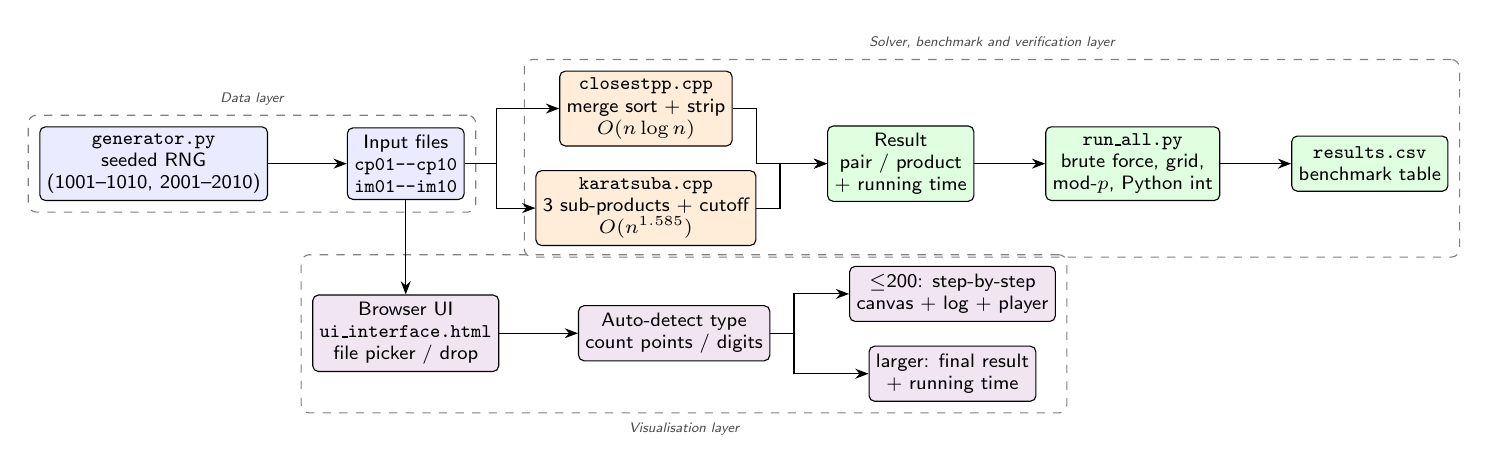
\begin{tikzpicture}[font=\scriptsize,>=Stealth,
  blk/.style={draw,rounded corners=2pt,align=center,minimum height=7mm,inner sep=2.5pt,fill=#1},
  blk/.default=white,
  grp/.style={draw,dashed,rounded corners=3pt,inner sep=4pt,gray},
  lab/.style={font=\tiny\itshape,gray!60!black}]
% data layer
\node[blk=blue!8] (gen) {\texttt{generator.py}\\seeded RNG\\(1001--1010, 2001--2010)};
\node[blk=blue!8,right=10mm of gen] (files) {Input files\\\texttt{cp01--cp10}\\\texttt{im01--im10}};
% C++ layer
\node[blk=orange!15,right=12mm of files,yshift=7mm] (cp) {\texttt{closestpp.cpp}\\merge sort + strip\\$O(n\log n)$};
\node[blk=orange!15,below=3mm of cp] (km) {\texttt{karatsuba.cpp}\\3 sub-products + cutoff\\$O(n^{1.585})$};
\node[blk=green!12,right=12mm of cp,yshift=-7mm] (out) {Result\\pair / product\\+ running time};
\node[blk=green!12,right=9mm of out] (ver) {\texttt{run\_all.py}\\brute force, grid,\\mod-$p$, Python int};
\node[blk=green!12,right=9mm of ver] (csv) {\texttt{results.csv}\\benchmark table};
% UI layer
\node[blk=violet!10,below=12mm of files,xshift=0mm] (ui) {Browser UI\\\texttt{ui\_interface.html}\\file picker / drop};
\node[blk=violet!10,right=10mm of ui] (det) {Auto-detect type\\count points / digits};
\node[blk=violet!10,right=10mm of det,yshift=5mm] (step) {$\le$200: step-by-step\\canvas + log + player};
\node[blk=violet!10,below=3mm of step] (big) {larger: final result\\+ running time};
% arrows
\draw[->] (gen)--(files);
\draw[->] (files.east)--++(4mm,0)|-(cp.west);
\draw[->] (files.east)--++(4mm,0)|-(km.west);
\draw[->] (cp.east)--++(3mm,0)|-(out.west);
\draw[->] (km.east)--++(3mm,0)|-(out.west);
\draw[->] (out)--(ver);
\draw[->] (ver)--(csv);
\draw[->] (files.south)--++(0,-3mm)-|(ui.north);
\draw[->] (ui)--(det);
\draw[->] (det.east)--++(3mm,0)|-(step.west);
\draw[->] (det.east)--++(3mm,0)|-(big.west);
% group frames
\begin{scope}[on background layer]
\node[grp,fit=(gen)(files),label={[lab]above:Data layer}] {};
\node[grp,fit=(cp)(km)(out)(ver)(csv),label={[lab]above:Solver, benchmark and verification layer}] {};
\node[grp,fit=(ui)(det)(step)(big),label={[lab]below:Visualisation layer}] {};
\end{scope}
\end{tikzpicture}
\end{document}
